\subsection{Application of Unknown Input Observer}
\label{sec:UIO_App}

\todo{discuss articles a bit}

The present chapter discusses how to apply unknown input observer (UIO) theory to the satellite functioning in nadir pointing control goal. The regular UIO uses linear model, however the satellite system is highly nonlinear.  During one orbit, the orientation of the nadir pointing satellite rotates by $360\deg$. By choosing the appropriate reference frame, this rotation can be eliminated from attitude dynamics. In local vertical, local horizontal frame (LVLH), the nadir pointing satellite keeps its attitude. This opens an opportunity to use linear approximation of the trigonometric nonlinearities in the satellite dynamic equations. The operating point should be chosen as nadir pointing, and if the attitude stays near enough to the operating point, the model stays quite accurate.

\todo{add LVLH to frames chapter}

Yang's article on desaturation \cite{DesatYang} describes a model that can be effective for UIO. The $\underline{A}$ matrix of the model is constant, so the UIO matrices can be derived as described in \ref{sec:UIO}. The model detaches the orbit angular velocity from the dynamics according to equation \ref{eq:angDetach}.

\begin{equation}
\label{eq:angDetach}
\vec{\omega} = \vec{_I^{lv}\omega} + \vec{_{lv}^s\omega}
\end{equation}

where $\vec{_I^{lv}\omega}$ is the angular velocity of the LVLH frame compared to the inertial frame and $\vec{_{lv}^s\omega}$ is the angular velocity of the body frame compared to the LVLH frame.

\todo{should we show the equations in more detail?}

\begin{align}
\begin{bmatrix}
\vec{_{lv}^s\dot{\omega}} \\
\vec{\dot{\omega}_{rw} } \\
\vec{\dot{q}_{1:3}}
\end{bmatrix}
 = 
\begin{bmatrix}
0 & 0 & \omega_o\frac{I_1 - I_2 + I_3}{-I_1} & 0 & 0 & \omega_o\frac{I_w}{-I_1} & 8\omega_o^2\frac{I_3 - I_2}{I_1} & 0 & 0 \\
0 & 0 &	0 & 0 & 0 &	0 & 0 &  6\omega_o^2\frac{I_3 - I_1}{I_2} & 0\\
 \omega_o\frac{I_1 - I_2 + I_3}{I_3}  & 0 & 0 &  \omega_o\frac{I_w}{I_3} & 0 &	0 & 0 & 0 & 2\omega_o^2\frac{I_1 - I_2}{I_3}\\
0 & 0 &	0  & 0 & 0 & 0 & 0 & 0 & 0\\
0 & 0 &	0  & 0 & 0 & 0 & 0 & 0 & 0 \\
0 & 0 &	0 & 0 & 0 & 0 & 0 & 0 & 0\\
0.5 & 0 &	0 & 0 & 0 & 0 & 0 & 0 & 0 \\
0 & 0.5 &	0& 0 & 0 & 0 & 0 & 0 & 0 \\
0 & 0 &	0.5 & 0 & 0 & 0 & 0 & 0 & 0\\
\end{bmatrix}
\begin{bmatrix}
_{lv}^s\omega_1 \\
_{lv}^s\omega_2 \\
_{lv}^s\omega_3 \\
\omega_{rw,1} \\
\omega_{rw,2} \\
\omega_{rw,3} \\
q_1 \\
q_2 \\
q_3 
\end{bmatrix}
 \\
+
\begin{bmatrix}
I_1^{-1} & 0 & 0 & 0 & \frac{b_3}{I_1} & -\frac{b_2}{I_1}\\
0 & I_2^{-1} & 0 & - \frac{b_3}{I_2} & 0 &  \frac{b_1}{I_2} \\ 
0 & 0 & I_3^{-1} &  \frac{b_2}{I_3} &  -\frac{b_1}{I_3} & 0 \\  
I_w^{-1} & 0 & 0 & 0 & 0 & 0 \\
0 & I_w^{-1} & 0 & 0 & 0 & 0 \\ 
0 & 0 & I_w^{-1} & 0 & 0 & 0 \\  
0 & 0 & 0 & 0 & 0 & 0 \\
0 & 0 & 0 & 0 & 0 & 0 \\
0 & 0 & 0 & 0 & 0 & 0 \\
\end{bmatrix}
\begin{bmatrix}
N_{rw,1} \\
N_{rw,2} \\
N_{rw,3}\\
\m_{mt,1} \\
\m_{mt,2} \\
\m_{mt,3} 
\end{bmatrix}
+
\begin{bmatrix}
N_{dist,1} \\
N_{dist,2} \\
N_{dist,3}\\
0\\
0\\
0\\
0\\
0\\
0
\end{bmatrix}
=
\underline{A}\vec{x} + \underline{B}(t)\vec{u} + \vec{d}
\label{eq:uioMatrices}
\end{align}

where $I_w$ is the reaction wheel axial moment of inertia, $\omega_o$ is the angular velocity of the orbit, $I_i$ is the satellite moment of inertia along $i$th principal axis.

\nomenclature[SIw]{$I_w$}{Reaction wheel axial moment of inertia}

\nomenclature[Somegao]{$\omega_o$}{Orbit angular velocity}

\begin{figure}[H]
	\centering
	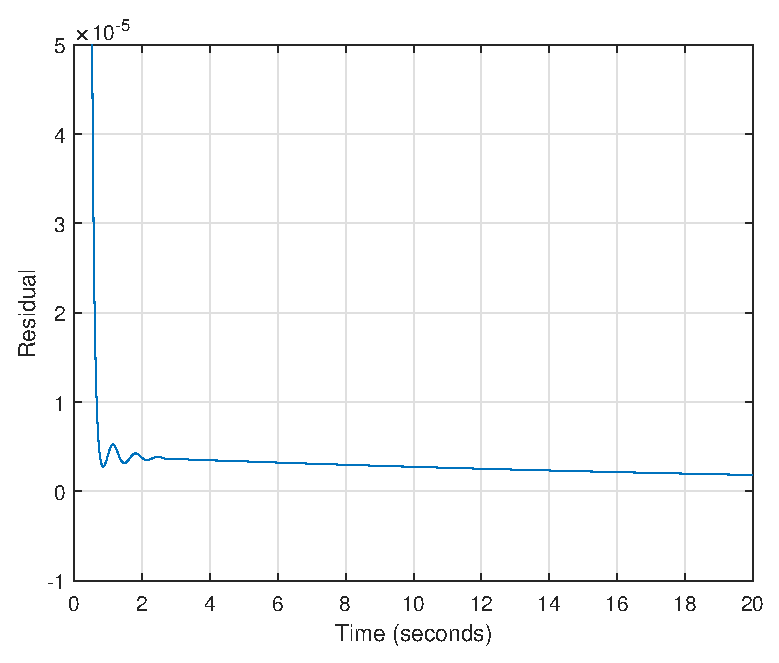
\includegraphics[width=0.7\linewidth]{figures/nosensfault_res}
	\caption{no sensor fault }
	\label{fig:}
\end{figure}

\begin{figure}[H]
	\centering
	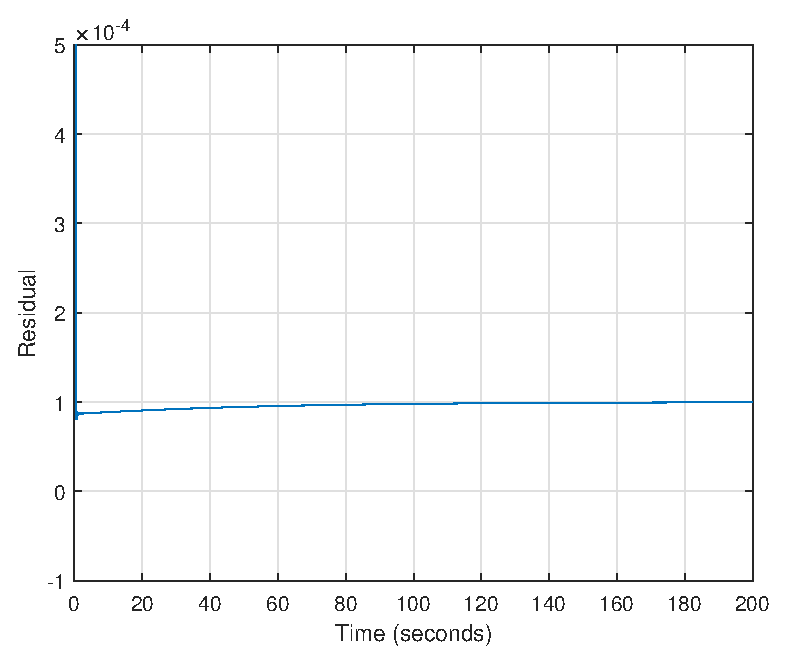
\includegraphics[width=0.7\linewidth]{figures/sensfault_res}
	\caption{sensor fault 0.1 ang vel x excess}
	\label{fig:}
\end{figure}

\begin{figure}[H]
	\centering
	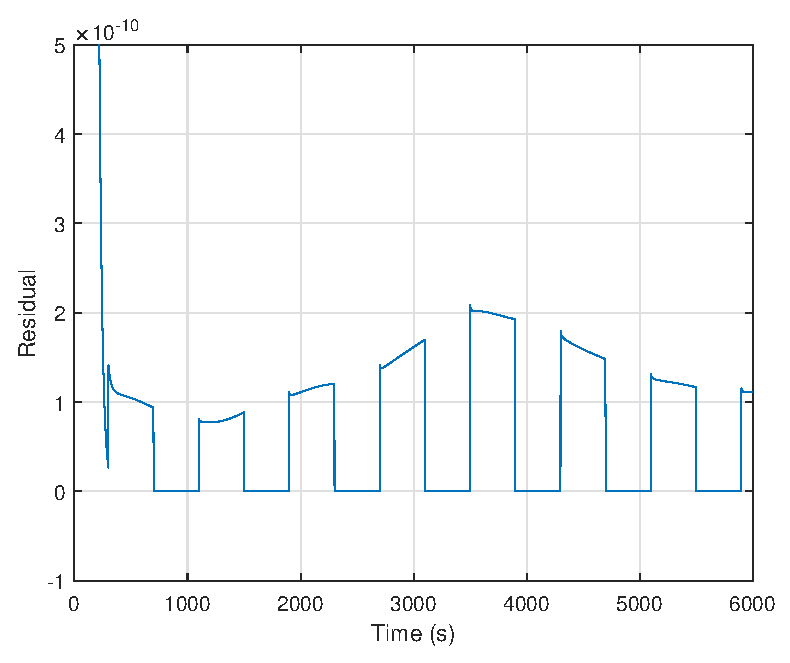
\includegraphics[width=0.7\linewidth]{figures/mt_fault_res}
	\caption{mmt error}
	\label{fig:residualmt}
\end{figure}

\begin{figure}[H]
	\centering
	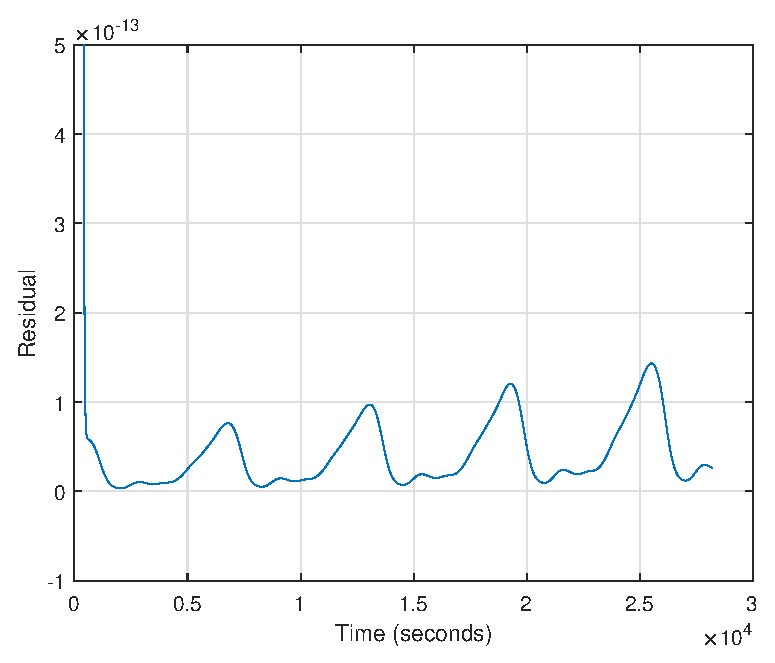
\includegraphics[width=0.7\linewidth]{figures/constdistonly_res}
	\caption{only dist const}
	\label{fig:residualdist}
\end{figure}

\begin{figure}[H]
	\centering
	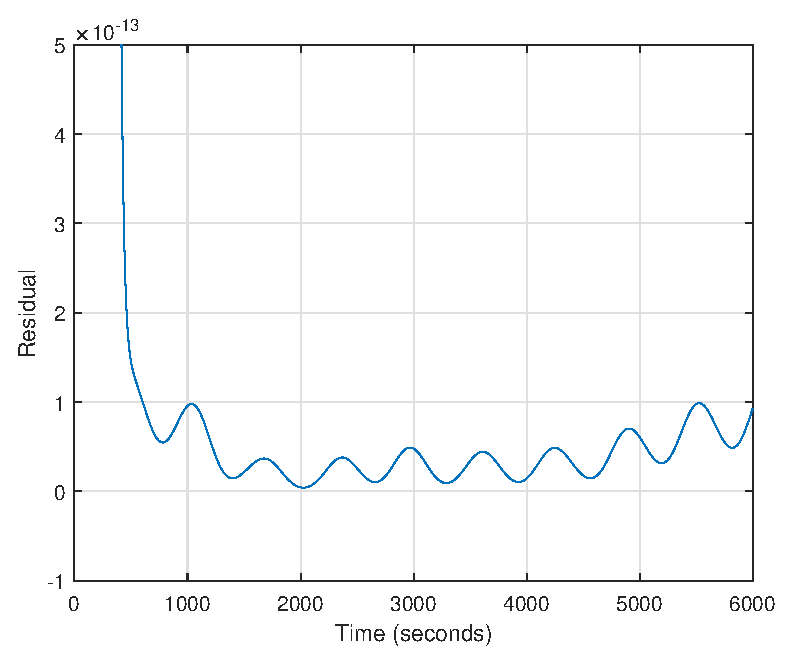
\includegraphics[width=0.7\linewidth]{figures/distonly_res}
	\caption{only dist sine}
	\label{fig:}
\end{figure}

%\nomenclature[Sw]{$\omega_o$}{Orbit angular velocity}
